\documentclass[12pt, a4paper]{article}

%\usepackage[cp1251]{inputenc}
\usepackage{a4wide} % уменьшает поля
\textwidth=12cm

\usepackage{background}
\SetBgScale{1}
\SetBgAngle{0}
\SetBgColor{black}
\SetBgContents{\rule{.4pt}{\paperheight}}
\SetBgHshift{4.5cm}

\usepackage{bm}

\usepackage[utf8]{inputenc}
\usepackage[russian]{babel} % включает русский язык
\usepackage{graphicx} % позволяет подключить .eps - файлы
\usepackage{amsmath}
\usepackage{amsthm} % теоремы от AMS
\usepackage{amssymb} % для работы с математическими R и проч.
\usepackage{floatrow}
\usepackage{mathrsfs}

\usepackage{accents}
\newcommand{\ubar}[1]{\underaccent{\bar}{#1}}

\newtheoremstyle{rusdef}
  {3pt}% measure of space to leave above the theorem. E.g.: 3pt
  {3pt}% measure of space to leave below the theorem. E.g.: 3pt
  {\itshape}% name of font to use in the body of the theorem
  {\parindent}% measure of space to indent
  {\bfseries}% name of head font
  {.}%
  {.5em}%
  {}

\theoremstyle{rusdef}
\newtheorem{definition}{Определение} % определение по-русски
\newtheorem{theorem}{Теорема}
\newtheorem{proposition}{Предложение}
\renewcommand\qedsymbol{$\blacksquare$}
\newtheorem{statement}{Утверждение}
\newtheorem{remark}{Замечание}
\newtheorem{lemma}{Лемма}
\newtheorem{corollary}{Следствие}
\newtheorem{assumption}{Предположение}
\newtheorem{example}{Пример}
\newtheorem{exersize}{Упражнение}

\newcommand\abs[1]{\left\lvert #1 \right\rvert} % модуль
\newcommand\bracket[1]{\left( #1 \right)} % скобки
\newcommand\scalar[1]{\left < #1 \right >} % скалярное произведение
\newcommand{\R}{\ensuremath{\mathbb{R}}} % R - мн-во вещественных чисел
\newcommand{\N}{\ensuremath{\mathbb{N}}} % N - мн-во натуральных чисел
\newcommand{\X}{\mathscr{X}} % красивая Х для начального и конечного множеств
\renewcommand{\P}{\mathscr{P}} % красивая P для ограничений на управление
\newcommand{\then}{\Rightarrow}
\newcommand{\h}{\mathbb{h}}
\newcommand{\e}{\mathbf{e}}

\renewcommand{\H}{\mathcal{H}} % красивая H для Гамильтона-Понтрягина
\newcommand{\M}{\mathcal{M}} % красивая M для Максимума
\renewcommand{\L}{\mathscr{L}} % красивая L для Лагранжа
\renewcommand{\d}{\partial} % чтобы долго не писать частную производную
\newcommand{\norm}[1]{\left\lVert #1 \right\rVert} % норма
\DeclareMathOperator*{\thus}{\Rightarrow} % следствие с возможностью использовать limits
\DeclareMathOperator*{\To}{\longrightarrow}
\DeclareMathOperator*{\Argmax}{Argmax} % Argmax с возмножностью использовать limits

\usepackage{indentfirst} % абзац после заголовка

\begin{document}

\parbox{11.8cm}{
  \begin{center}
    {\Huge Доказательство принципа максимума и модель Рамсея}
  \end{center}
}

\section*{Задачи на принцип максимума}
Задачи из этой секции обязательно прорешать при подготовке к экзамену!

\begin{exersize}
  \[ J = x_2(1) \to \max \]
  \[
    \left\{
    \begin{aligned}
      \dot{x}_1 & = -u_1 x_1 + u_1^2 x_2,  \\
      \dot{x}_2 & = u_2 x_1 - 3 u_1^2 x_2,
    \end{aligned}
    \right.
    \qquad
    \begin{matrix}
      |u_1| \leqslant 1 \\
      |u_2| \leqslant 1
    \end{matrix}
  \]
\end{exersize}

\begin{exersize}
  \[ J = \int\limits_0^1 \left[ u_1^2 + x_1 x_2 - u_2 \right] dt + x_1(0) x_2(0) - x_1(1) x_2^2(0) \to \inf \]
  \[
    \left\{
    \begin{aligned}
      \dot{x}_1 & = x_1 + u_1 x_2, \\
      \dot{x}_2 & = u_2 x_1,
    \end{aligned}
    \right.
    \qquad
    \begin{matrix}
      |u_1| \leqslant 1 \\
      |u_2| \leqslant 1
    \end{matrix}
  \]
\end{exersize}

\textit{PS. Изначально этот раздел был в самом конце, но я изменил компоновку, чтобы вы точно его увидели. \textbf{Обязательно} научитесь решать такие задачи, на экзамене по крайней по одной такой будет у каждого.}

\section{Абстрактная задача нелинейного программирования (АЗНЛП)}

Пусть задано некоторое множество произвольной природы. \textit{Например, это множество специй, которые Вы собираетесь добавить в суп}.

Рассмотрим следующую задачу минимизации:
\[
  \left\{
  \begin{aligned}
    J_0(s) & \to \inf, \quad  s \in S,       \\
    J_1(s) & = J_2(s) = \ldots = J_3(s) = 0.
  \end{aligned}
  \right.
\]

Идея для построение решения задачи в такой постановке: ввести конечномерную параметризацию.

Пусть $s^* \in S$ "--- оптимальная точка, $\bar{J} = [J_0, J_1, \ldots, J_k]^T$. Пусть некоторые параметры $\rho = (\rho_1, \ldots, \rho_{k+1})$ заданы таким образом, что для всех элементов $s$ из окрестности $s^*$ выполнено
\[
  s = \zeta(\rho), \quad s^* = \zeta(0).
\]
При этом при выборе параметризации подберём $\zeta(\cdot)$ таким образом, чтобы значения параметров $\rho_i$ были неотрицательными:
\[
  \rho_i \geqslant 0, \quad i = 1, \ldots, k+1.
\]

Запишем ограничения, накладываемые на описанную параметризацию, более формально.

Пусть $e_1, \ldots, e_{k+1}$ "--- стандартный ОНБ в $\R^{k+1}$, \textit{то есть \\ ${e_i = (0,\ldots,0,1,0,\ldots,0)^T}$, где 1 стоит на i-ом месте}. Рассмотрим симплекс следующего вида:
\[
  C = \mathrm{conv} \left\{ (0,\ldots,0)^T, e_1, \ldots, e_k \right\}
\]

\begin{figure}[ht]
  \center
  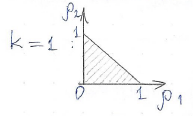
\includegraphics{pic1.png}
\end{figure}

Тогда, ввиду нашего требования неотрицательности для $\rho_i$,
\[
  \exists \eta > 0\colon \quad \rho \in \eta C,
\]
где $\eta C = \mathrm{conv} \left\{ (0,\ldots,0), \eta e_1, \ldots, \eta e_k \right\}$;

Тогда $\zeta \colon \eta C \to S$. Чаще всего удаётся построить непрерывную параметризацию $\zeta(\cdot)$, но, вообще говоря, непрерывной она быть не обязана.

Непрерывность мы потребуем от $\bar{J}(\zeta(\cdot))$ "--- эта функция обязательно должна быть непрерывной в $\eta C$. Свойства же каждой из двух функций нам, вообще говоря, не важны.

\begin{definition}
  $\bar{M} \in \R^{(k+1) \times (k+1)}$ "--- конический дифференциал от $\bar{J}$ в $s^*$ вдоль $\zeta(\rho)$, если
  \[
    \bar{J}(\zeta(\rho)) = \bar{J}(\zeta(0)) + \bar{M}\rho + \bar{o}(\| \rho \|).
  \]
\end{definition}

\begin{definition}
  Конус $\bar{K} \subseteq \R^{k+1}$ "--- конус вариации $\bar{J}$ в $s^*$, если для любых линейно-независимых векторов
  ${\forall \bar{d}^1, \ldots, \bar{d}^{k+1} \in \bar{K}}$ ${\exists \; \eta > 0, \zeta \colon}$
  \[
    \bar{M} =
    \begin{bmatrix}
      |         &        & |             \\
      \bar{d}^1 & \ldots & \bar{d}^{k+1} \\
      |         &        & |
    \end{bmatrix}
    \quad \text{ "--- конический дифференциал}.
  \]
\end{definition}

\begin{theorem}[абстрактное правило множителей Лагранжа]
  Пусть $s^* \in S$, $s^*$ "--- решение АЗНЛП, то есть
  \[
    J_1(s^*) = \ldots = J_k(s^*) = 0, \quad J_0(s^*) \leqslant J_0(s) \: \forall s \in S.
  \]
  Пусть $\bar{K}$ "--- \textbf{выпуклый} конус вариаций в $s^*$.

  Тогда существует ${\exists\, \bar{\lambda} = (\lambda_0, \ldots, \lambda_k)^T \neq 0}$ такой, что ${\lambda_0 \leqslant 0}$ и
  \[
    {\left< \bar{\lambda}, \bar{d} \right>} \leqslant 0, \: \forall \bar{d} \in \bar{K}
  \]
\end{theorem}

\begin{proof}[Идея доказательства]
  Рассмотрим
  \[
    \bar{l} = \left\{ \bar{y} \in \R^{k+1}, \; y_0 \leqslant 0, y_1 = \ldots = y_k = 0 \right\}.
  \]

  $\bar{K}$ и $\bar{l}$ отделимы, то есть
  \[
    \exists \bar{\lambda} \neq 0 \colon \forall \bar{y} \in \bar{l} \:\forall
    \bar{d} \in \bar{K} \thus \left< \bar{\lambda}, \bar{d} \right> \leqslant 0 \leqslant \left< \bar{\lambda}, \bar{y} \right>,
  \]
  поскольку $0 \in \bar{l} \cap \bar{K}$. При этом $\left< \bar{\lambda}, \bar{y} \right> = \lambda_0 y_0 \geqslant$, что, совместно с условием $y_0 \leqslant 0$, даёт нам $\lambda_0 \leqslant 0$.

  Если они не отделимы, то найдётсся $s$, удовлетворяющее ограничениям, такое, что $J_0(s) < J_0(s^*)$.
\end{proof}
%   Предположим противное: пусть $\bar{K}$ и $\bar{l}$ не отделимы, тогда $(-1,0,\ldots,0)^T \in \mathrm{int} \bar{K}$ (иначе бы $0 \in \d \bar{K}$). Тогда \[B_{\varepsilon}((-1,0,\ldots,0)^T) \subset \mathrm{int} \bar{K}.\]

%   Проведём гиперплоскость $y_0 = -1$, рассмотрим симплекс $D \subseteq \left\{ \bar{y} \colon y_0 = -1 \right\}$, $(-1,0,\ldots,0)^{-1} \in \mathrm{ri} D$.

%   $D = \mathrm{conv} \left\{ \bar{d}^1, \bar{d}^2, \ldots, \bar{d}^{k+1} \right\}$, $\bar{d}^1, \ldots, \bar{d}^{k+1}$ "--- линейно независимые.

%   \[
%     \bar{M} =
%     \begin{bmatrix}
%       |         &        & |             \\
%       \bar{d}^1 & \ldots & \bar{d}^{k+1} \\
%       |         &        & |
%     \end{bmatrix}, \quad
%     \,\exists\, \gamma > 0, \,\exists\,\zeta(\cdot) \colon |\bar{M}| \neq 0.
%   \]

%   $\bar{M}$ "--- конический дифференциал $\bar{J}$, $\zeta \colon \gamma C \to S$.

%   Рассмотрим $\Delta = \mathrm{conv} \left\{ 0, \bar{d}^1, \ldots, \bar{d}^{k+1} \right\}$.
%   \[
%     \bar{J}(\zeta(\rho)) = \bar{J}(s^*) + \bar{M} \rho + \bar{o}(\|\rho\|), \: \rho \in \gamma C,
%   \]
%   \[
%     \bar{M}(\gamma C) = \gamma \Delta.
%   \]

%   Рассмотрим $\Psi(\bar{y}) = \bar{J}\left( \zeta(\bar{M}^{-1}\bar{y}) \right) - \bar{J}(s^*), \bar{y} \in \gamma\Delta$. $\bar{y} = \bar{M} \rho \thus$ ${\rho = \bar{M}^{-1} \bar{y}}$.

%   Требуется найти $s \in S \colon J_0(s) < J_0(s^*)$ такое, что \\ ${J_1(s) = \ldots = J_k(s) = 0}$. Эту задачу мы свели к поиску $\bar{y}$ такого, что 
% \end{proof}

\section{Доказательство принципа максимума}

Итак, $s = \left\{ t_0, t_1, x^0, u(\cdot) \right\} \in S$. $u^*$ является кусочно"=непрерывной, в точке $t = t_0$ "--- непрерывной справа и всюду непрерывной слева.

Выписываем в привычном нам виде $e = (t_0, x^0, t_1, x^1)$, \\ $\varphi_0(e) \to \min$, $\varphi_1(e) = \ldots = \varphi_k(e) = 0$,
\[
  \bar{\varphi} =
  \begin{bmatrix}
    \varphi_0 \\ \varphi_1 \\ \ldots \\ \varphi_k
  \end{bmatrix},
  \quad
  s^* = \{ t_0^*, t_1^*, x^{0*}, u^*(\cdot) \}.
\]

\begin{theorem}
  Пусть $e^* = (t_0^*, x^{0*}, t_1^*, x^{1*})$. Определим векторы
  \begin{enumerate}
    \item[(i)] $\pm \left[ \dfrac{\d \bar{\varphi}}{\d t_0} + \dfrac{\d \bar{\varphi}}{\d x^0}(e^*) f(t_0^*, x^*(t_0^*), u^*(t_0^*)) \right]$;
    \item[(ii)] $\pm \left[ \dfrac{\d \bar{\varphi}}{\d t_1} + \dfrac{\d \bar{\varphi}}{\d x^1}(e^*) f(t_1^*, x^*(t_1^*), u^*(t_1^*)) \right]$;
    \item[(iii)] $\dfrac{\d \bar{\varphi}}{\d x^0}(e^*) \delta x^0 + \dfrac{\d \bar{\varphi}}{\d x^1}(e^*) \delta x^{(0)} (t_1^*)$, где 
    \[
      \left\{
        \begin{aligned}
          \dfrac{d}{dt}\delta x^{(0)}(t) &= \dfrac{\d f}{\d x}(t, x^*(t), u^*(t)) \delta x^{(0)}(t), \\
          \delta x^{(0)} (t^*_0) &= \delta x^0;
        \end{aligned}
      \right.
    \]
    \item[(iv)] $\dfrac{\d \bar{\varphi}}{\d x^1}(e^*) \delta x(t_1^*)$, где
    \[
      \left\{
        \begin{aligned}
          \dfrac{d}{dt}\delta x(t) &= \dfrac{\d f}{\d x}(t, x^*(t), u^*(t)) \delta x(t), \\
          \delta x (\tau) &= f(\tau, x^*(\tau), v) - f(\tau, x^*(\tau), u^*(\tau));
        \end{aligned}
      \right.
    \] 
  \end{enumerate}

  Тогда выпуклый конус $\bar{K}$, порождённый $(i), (ii), (iii), (iv)$, является конусом вариаций.
\end{theorem}
\begin{proof}
  Без доказательства.
\end{proof}

\begin{remark}
  Эти вариации получены при варьировании каждой из $\bar{\varphi}(e^*) = \bar{t_0^*, x^{0*}, t_1^*, x^{1*}}$. \\
  $(i)$ и $(ii)$ "--- проварьировали $t_0 = t_0^* + \delta t_0$ и $t_1 = t_1^* + \delta t_1$ соответственно. \\
  $(iii)$ получается при варьировании $x^0 = x^{0*} + \delta x^0$ аналогично тому, как мы делали в доказательстве теоремы о зависимости от начальных параметров; отсюда и такая знакомая и похожая система на вариацию. \\
  $(iv)$ "--- проварьировали по $x^1$, что возможно только при варьировании управления. Отсюда здесь возникает $\tau$ "--- это момент времени, в который мы подставили <<иголку>>. Используя игольчатую вариацию, получим соответствующее изменение $x^1$, которое мы варьируем в $\bar{\varphi}$.
\end{remark}

Теперь мы готовы доказать принцип максимума, сформулированный в прошлый раз.

\begin{theorem}
  Пусть $\{x^*(\cdot), u^*(\cdot)\}$ "--- оптимальная пара с $e^* = (t_0^*, x^{0*}, t_1^*, x^{1*})$. Тогда \ldots (ПМП).
\end{theorem}
\begin{proof}
  По абстрактному правилу множителей\\ Лагранжа $\exists \bar{\lambda} = (\lambda_0, \lambda_1, \ldots, \lambda_K)^T \neq 0 \colon$
  \[
    \lambda_0 \leqslant 0, \left< \bar{\lambda}, \bar{d} \right> \leqslant 0 \quad \forall \bar{d} \in \bar{K}.
  \]
  Обозначим (СС):
  \[
    \dot{\psi}^*(t) = - \left. \dfrac{\d \H}{\d x} \right\vert_{\ldots} = - \left[ \dfrac{\d f(t, x^*(t), u^*(t))}{\d x} \right]^T \psi^*(t),
  \]
  начальное условие (одно из УТ)
  \[
    \psi^*(t_1^*) = \left( \dfrac{\d \varphi(e^*)}{\d x^1} \right)^T \bar{\lambda}
  \]

  Для любого $\tau \in (t_0^*, t_1^*), \; \forall v \in \P\colon$
  \[
    \dfrac{d}{dt} \left< \psi^*(t), \delta x(t) \right> = \left< - \left[\dfrac{\d f}{\d x}\right]^T \psi^* , \delta x(t)\right> + \left<\psi^*, \left[\dfrac{\d f}{\d x}\right] \delta x \right> = 0.
  \]
  \[
    \left< \psi^*(t_1^*), \delta x(t_1*) \right> = \left< \psi^*(\tau), \delta x(\tau) \right>.
  \]
  Поскольку (из (iv)):
  \[
    \psi^*(t_1^*) = \left[ \dfrac{\d \bar{\varphi}(e^*)}{\d x^1} \right]^T \bar{\lambda} = \left< \bar{\lambda}, \left[ \dfrac{\d \bar{\varphi}}{\d x^1} \right] \delta x(t_1^*) \right> = \left<\bar{\lambda}, \bar{d}\right> \leqslant 0,
  \]
  а
  \[
    \delta x(\tau) = f(\tau, x^*(\tau), v) - f(\tau, x^*(\tau), u^*(\tau)),
  \]
  отсюда получаем (УМ):
  \[
    \left< \psi^*(\tau), f(\tau, x^*(\tau), v) \right> \leqslant \left< \psi^*(\tau), f(\tau, x^*(\tau), u^*(\tau)) \right>.
  \]

  Аналогично $\dfrac{d}{dt} \left< \psi^*(t), \delta x^{(0)}(t) \right> = 0$, $\delta x^{(0)}(t_0^*) = \delta x^0$,
  \[
    \psi^*(t_1^*) = \left[\dfrac{\d \bar{\varphi}}{\d x^1}\right]^T \bar{\lambda} = \left<\bar{\lambda}, \dfrac{\d \bar{\varphi}}{\d x^1} \delta x^{(0)}(t_1^*) \right>
  \]
  Подставив эти значения и прибавив в обоих частях выражение $\left< \bar{\lambda}, \dfrac{\d \bar{\varphi}}{\d x^0} \delta x^0 \right>$, получим (с учётом (iii)):
  \[
    \left< \psi^*(t_0^*), \delta x^0 \right> + \left< \left[\dfrac{\d \bar{\varphi}}{\d x^0}\right]^T ,\delta x^0 \right> = \left< \bar{\lambda}, \dfrac{\d \bar{\varphi}}{\d x^1} \delta x^{(0)}(t_1^*) + \dfrac{\d \bar{\varphi}}{\d x^0} \delta x^0 \right> \!\leqslant\! 0.
  \]
  То есть
  \[
    \left< \psi^*(t_0^*) + \left[\dfrac{\d \bar{\varphi}}{\d x^0}\right]^T \bar{\lambda}, \delta x^0 \right> \leqslant 0, \quad \forall \delta x^0 \in \R^n.
  \]
  Положим $\psi^*(t_0^*) = -\left[\dfrac{\d \bar{\varphi}}{\d x^0}\right]^T \bar{\lambda}$, получим второе условие трансверсальности.

  Пусть теперь $j = 0, 1$. Используем (i) и (ii), из них следует, что $\left<\bar{\lambda}, \bar{d} \right> \leqslant 0$, и одновременно с этим $\left<\bar{\lambda}, -\bar{d} \right> \leqslant 0$, то есть $\left<\bar{\lambda}, \bar{d} \right> = 0$.

  Тогда
  \[
    \left< \bar{\lambda}, \dfrac{\d \bar{\varphi}(e^*)}{\d t_j} + \dfrac{\d \bar{\varphi}(e^*)}{\d x^j} f(t_j^*, x^*(t_j^*), u^*(t_j^*)) \right> = 0.
  \]
  Подставляя в
  \[
    \left< \dfrac{\d \bar{\varphi}(e^*)}{\d t_j}, \bar{\lambda} \right> + \left< \left[\dfrac{\d \bar{\varphi}(e^*)}{\d x^j}\right]^T \bar{\lambda}, f(t_j^*, x^*(t_j^*), u^*(t_j^*)) \right> = 0
  \]
  значения
  \begin{gather*}
    \left[\dfrac{\d \bar{\varphi}(e^*)}{\d x^0}\right]^T \bar{\lambda} = -\psi^*(t_0^*),\\
    \left[\dfrac{\d \bar{\varphi}(e^*)}{\d x^1}\right]^T \bar{\lambda} = \psi^*(t_1^*),
  \end{gather*}
  получим (УТ) по времени.

  Мы доказали принцип максимума.
\end{proof}

Пусть теперь $\exists\, \dfrac{\d f}{\d t}$. Существует ли производная 
\[
  \dfrac{d}{dt} \H(t, x^*(t), \psi^*(t), u^*(t))?
\]
Рассмотрим $h(t, v) = \left< \psi^*(t), f(t, x^*(t), v) \right>$. Эта функция непрерывна по $t$ и, в силу (УМ),
\[
  \max\limits_{v \in \P} h(t,v) = h(t, u^*(t)),
\]
$u^*$ "--- кусочно-непрерывная, непрерывная слева.
$\forall t \in (t_0^*, t_1^*)$ подберём $\Delta t \colon t + \Delta t \in (t_0^*, t_1^*)$. Тогда
\begin{gather*}
  h(t, u^*(t + \Delta t)) \leqslant h(t, u^*(t)), \\
  h(t + \Delta t, u^*(t)) \leqslant h(t + \Delta t, u^*(t + \Delta t)).
\end{gather*}
Устремляем $\Delta t \to 0$:
\[
  h(t, u^*(t \pm 0)) \leqslant h(t, u^*(t)) \leqslant h(t, u^*(t \pm 0)),
\]
то есть $h(t, u^*(t))$ "--- непрерывна по $t$.

Снова воспользуемся свойством $h$: при $\Delta t > 0$
\begin{gather*}
  \Delta h = h(t + \Delta t, u^*(t + \Delta t)) - h(t, u^*(t)) \;\thus \\
  \Delta h \leqslant h(t + \Delta t, u^*(t + \Delta t)) - h(t, u^*(t + \Delta t)), \\
  \Delta h \geqslant h(t + \Delta t, u^*(t)) - h(t, u^*(t)).
\end{gather*}
Пусть $t$ "--- точка непрерывности $u^*(\cdot)$ (такие точки п.в.), тогда можем оба неравенства разделить на $\Delta t \to 0$ и получить
\[
  \dfrac{d}{dt} h(t, u^*(t)) = \dfrac{\d h(t, u^*(t))}{\d t} = \left. \dfrac{\d h(t, v)}{\d t} \right\vert_{v = u^*(t)}.
\]
Таким образом, перешли от полной производной к частной.

С другой стороны,
\begin{multline*}
  \dfrac{\d h}{\d t} = \left< - \left[\dfrac{\d f}{\d x}\right]^T \psi^*(t), f(t, x^*(t), v) \right> +
  \left< \psi^*(t), \dfrac{\d f}{\d t}(t, x^*(t), v) \right> + \\ +
  \left< \psi^*(t), \dfrac{\d f}{\d x} f(t, x^*(t), u^*(t)) \right>.
\end{multline*}

Приводя слагаемые, получаем
\[
  \left. \dfrac{\d h}{\d t} \right\vert_{v = u^*(t)} = \left< \psi^*(t), \dfrac{\d f}{\d t} (t, x^*(t), u^*(t)) \right>.
\]

\begin{corollary}
  \begin{multline*}
    \H(t, x^*(t), \psi^*(t), u^*(t)) = \H(t_0^*, x^*(t_0^*), \psi^*(t_0^*), u^*(t_0^*)) + \\
    + \int\limits_{t_0^*}^{t} \left< \psi^*(\tau), \dfrac{\d f}{\d t} (\tau, x^*(\tau), u^*(\tau)) \right> d\tau.
  \end{multline*}
  Кроме того, в случае, когда система автономная, последний интеграл равен нулю, откуда следует $\H \equiv \mathrm{const}$.
\end{corollary}

\section{Модель Рамсея}
Рассмотрим классическую модель из области мат.~экономики "--- модель Рамсея. На её примере мы продемонстрируем, как абстрактное правило множителей Лагранжа может применяться к решению задач управления.

Введём необходимые обозначения.

$K$ "--- капитал, объём основных фондов. \textit{Не ограничивается только деньгами. Например, если денег во время карантина у Вашей организации много, но Вы снабжаете сотрудников одноразовыми масками, чтобы они могли работать, количество масок станет для Вас важным ресурсом, за которым Вы будете следить}.

$L$ "--- люди, рабочая сила.

Производственная функция определена как
\[ Y = \mathcal{F}(K, L) \]
и представляет собой величину, на которую за единицу времени растёт капитал $K$ при фиксированных значениях $(K, L)$. Это значение мы разделим на две разные по смыслу части: инвестиции в производство $I$ и потребление $C$ \textit{(по сути это и есть наш доход)}:
\[ Y = I + C \]

В этой системе управлять мы будем долей $Y$, возвращаемой обратно в производство:
\[ I = u\mathcal{F}, \qquad C = (1-u)\mathcal{F}, \qquad 0 \leqslant u \leqslant 1. \]

Пусть, кроме того, в процессе производства происходит амортизация, определяемая коэффициентом $\mu >0$.

Запишем систему дифференциальных уравнений, описывающую функционирование описанной динамической системы.
\[
  \left\{
  \begin{aligned}
    \dfrac{dK}{dt} & = \mathcal{F}(K, L)u(t) - \mu K, \\
    C(t)           & = (1-u(t))\mathcal{F}(K,L).
  \end{aligned}
  \right.
\]

Мы будем предполагать, что производственная функция $\mathcal{F}$ удовлетворяет следующим ограничениям:
\[
  \frac{\d \mathcal{F}}{\d \mathcal{F}} > 0, \quad \frac{\d F}{\d L} > 0, \quad \mathcal{F}(\alpha K, \alpha L) = \alpha \mathcal{F}(K, L), \; \alpha > 0.
\]
Первые два условия следуют из интерпретации: мы ожидаем, что если мы увеличим доступный нам капитал или же рабочую силу (наймём дополнительных сотрудников, например), то объёмы производства вырастут. Свойство положительной однородности определяет характер этого роста \textit{(в данном случае, прирост будет линейным: например, если мы в 2 раза увеличим количество касс в метро и посадим за них в 2 раза больше билетёров, то они смогут продавать в 2 раза больше билетиков в единицу времени)}.

Введём переобозначения, которые упростят нашу систему.

Пусть $k = \dfrac{K}{L}$ "--- удельный капитал \textit{(капитал на единицу рабочей силы)}, $c = \dfrac{C}{L}$ "--- доход на душу. Тогда
\[
  \dfrac{\mathcal{F}(K,L)}{L} = \mathcal{F}(k, 1) \equiv f(k), \qquad c = \dfrac{C}{L} = (1-u)f(k).
\]
Тогда получим систему дифференциальных уравнений следующего вида:
\[
  \left\{
  \begin{aligned}
    \dot{k} & = uf(k) - \mu k,   \\
    c(t)    & = (1-u(t))f(k(t)), \\
    k(0)    & = k_0 > 0.
  \end{aligned}
  \right.
\]

Условия на $f$:
\begin{enumerate}
  \item $f \in C^2, \quad k > 0$; $f(+\infty) = +\infty$;
  \item $f(0) = 0, \quad f'(k) > 0, k > 0$; $f'(+0) = +\infty, \; f'(+\infty) = 0$;
  \item $f''(k) < 0, k > 0$.
\end{enumerate}

Пример производственной функции: функция Кобба-Дугласа
\[f(k) = k^{\alpha}, \quad 0 < \alpha < 1,\]
где $\alpha$ "--- коэффициент эластичности.

Перейдём непосредственно к постановке задачи управления.

Пусть $t \in [0, T] \thus k(T) \geqslant k_T > 0$. Будем решать задачу вида
\[
  \int\limits_{0}^{T} \e^{-\rho t} c(t) dt \to \max,
\]
то есть стремиться постоянно поддерживать максимальный уровень доходов (а не только в конечный момент времени). Здесь $\rho > 0$ "--- коэффициент дисконтирования, а $\e^{-\rho t}$ "--- дисконтирующий множитель. Он всюду убывает и имеет следующую интерпретацию: чем дальше время получения прибыли, тем менее она для нас ценна. \textit{Это может показаться немного странным, поэтому приведём пример. Представьте, что Вы заняли 200 рублей другу. Если он вернёт деньги завтра "--- считайте, что и не заметили. Если он вернёт их через месяц "--- уже немного неприятно, на них можно было сходить пообедать не в столовую, а куда-то ещё, но пришлось идти в столовую. Если Вы получите эти деньги через год, то, считайте, что они уже почти ничего не стоят "--- сегодня на них можно купить бизнес-ланч, а через год только половину бизнес-ланча. Так и работает дисконтирование "--- чем более отдалена дата выплаты, тем меньшую ценность для нас имеет одна и та же сумма}.

Вернёмся к нашей задаче.
\[
  \left\{
    \begin{aligned}
      &\dot{k} = uf(k) - \mu k, \\
      &k(0) = k_0, \: k(T) \geqslant k_T > 0, \\
      &J = \int_0^T \e^{-\rho t} (1-u)f(k) dt \to \max.
    \end{aligned}
  \right.
\]

Обобщим её:
\begin{gather*}
  \dot{x} = f(x, u), \\
  \int_{t_0}^{t_1} \e^{-\rho t} f^0(x, u) dt \to \max.
\end{gather*}


Функция Гамильтона-Понтрягина для этой задачи:
\begin{multline*}
  \H = \psi_0 \e^{-\rho t}f^0(x,u) + \left<\psi, f(x,u) \right> = \\ = \e^{-\rho t} \left( \psi_0 f^0(x,u) + \left< \psi \e^{\rho t}, f(x,u) \right> \right) = \\ = \e^{-\rho t} \left( \eta_0 f^0(x,u) + \left< \eta, f(x,u) \right> \right) = \e^{-\rho t} \tilde{\H}.
\end{multline*}

Таким образом, мы перешли от сопряжённых переменных
\[
  \left\{
    \begin{aligned}
      \dot{\psi}_0 &= 0, \\
      \dot{\psi} &= -\psi_0\e^{-\rho t} \dfrac{\d f^0}{\d x} - \left(\dfrac{\d f}{\d x}\right)^T \psi,
    \end{aligned}
  \right.
\]
к переменным
\[
  \left\{
    \begin{aligned}
      \dot{\eta}_0 &= 0, \\
      \dot{\eta} &= \rho \eta - \eta_0 \dfrac{\d f^0}{\d x} - \left(\dfrac{\d f}{\d x}\right)^T \eta.
    \end{aligned}
  \right.
\]

В терминах нашей исходной системы (на $k(\cdot)$):
\[
  \tilde{\H} = \eta_0 (1 - u)f(k) + \eta(uf(k) - \mu k),
\]
(СС) имеет вид:
\[
  \left\{
    \begin{aligned}
      \dot{\eta}_0 &= 0, \\
      \dot{\eta} &= \rho \eta - \eta_0 (1 - u)f'(k) - \eta (u f' - \mu).
    \end{aligned}
  \right.
\]

\subsubsection*{Нормальный случай}
\[
  \eta_0 = 0 \thus \qquad
  u =
  \left\{
    \begin{aligned}
      1, &\quad \eta > 1, \\
      [0,1], &\quad \eta = 1, \\
      0, &\quad \eta  < 1.
    \end{aligned}
  \right.
\]
\[
  \begin{gathered}
    \bm{\eta > 1 \colon}\\
    \left\{
      \begin{aligned}
        \dot{k} &= f(k) - \mu k, \\
        \dot{\eta} &= \eta(\rho - f' + \mu)
      \end{aligned}
    \right.
  \end{gathered}
  \qquad \qquad
  \begin{gathered}
    \bm{\eta < 1 \colon}\\
    \left\{
      \begin{aligned}
        \dot{k} &= \mu k, \\
        \dot{\eta} &= \eta(\rho + \mu) - f'.
      \end{aligned}
    \right.
  \end{gathered}
\]

Особый режим? Пусть $\eta = 1$ на $[t_1, t_2]\colon$
\begin{gather*}
  0 = \dot{\eta} = \rho - (1-u)f' - uf' + \mu \thus f' = \rho + \mu \\
  \thus \,\exists!\, k^* \colon f'(k^*) = \rho + \mu \;\thus\; k = \mathrm{const} \\
  \thus\; 0 = \dot{k} = u f(k^*) - \mu k^* \;\thus\; u_{oc} = \dfrac{\mu k^*}{f(k^*)}
\end{gather*}
По условию $u \leqslant 1 \thus u_{oc} \leqslant 1 \thus \mu k^* \leqslant f(k^*)$. Выполняется ли это условие?


Рассмотрим $\bar{k} \colon f(\bar{k}) = \mu \bar{k}$. Оно существует поскольку
\[
  f(k) - \mu k \To\limits_{k \to +\infty} -\infty, \qquad f'(k) - \mu \To\limits_{k \to +\infty} - \mu,
\]

\begin{figure}[ht]
  \center
  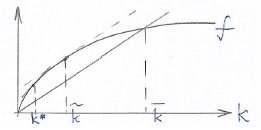
\includegraphics{pic2.png}
\end{figure}

$\exists \tilde{k} \colon\: f'(\tilde{k}) = \mu \colon\: \bar{k} > \tilde{k} > k^*$.

$f'(k^*) > \mu \:\thus\: \mu k^* < f(k^*)$, то есть $u_{oc} < 1$.

Типичным при решении задач является случай, когда
\[
  k_0, k_T < \bar{k}, \qquad (k(0) = k_0, \quad k(T) \geqslant k_T > 0).
\]

\begin{figure}[ht]
  \center
  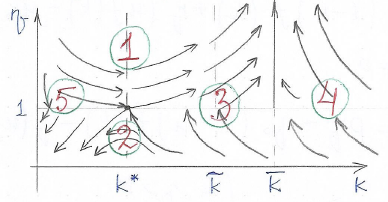
\includegraphics{pic3.png}
\end{figure}

\begin{enumerate}
  \item[1:] 
  \begin{align*}
    &\dfrac{dk}{dt} = f(k) - \mu k, \\
    &\dfrac{dk}{f(k) - \mu k} = dt \;\thus\: T_1 = \int\limits_{k_0}^{k_T} \dfrac{dk}{f(k)} - \mu k
  \end{align*}
  \item[2:] $k_0 \leqslant k_T$,
  \[
    \dot{k} = - \mu k \;\thus\: \dfrac{dk}{\mu k} = -dt \;\thus\: T_2 = \int\limits_{kT}^{k_0} \dfrac{dk}{\mu k}
  \]
  \item[3:] Аналогично
  \[
    T_3 = \int\limits_{k_*}^{k_0}\dfrac{dk}{\mu k} + \int\limits_{k^*}^{k_T} \dfrac{dk}{f(k) - \mu k}
  \]
  \item[5:]
  \[
    T_5 = \int\limits_{k_0}^{k^*} \dfrac{dk}{f(k) - \mu k} + \int\limits_{k_T}^{k^*}\dfrac{dk}{\mu k}
  \]  
\end{enumerate}
Обозначим $\bar{T} = \max(T_1, T_2, T_3, T_5)$.

На основании всего проведённого исследования системы, можем сформулировать следующий результат.
\begin{theorem}
  Если $T > \bar{T}$, то существуют $\tau_1 < \tau_2 \colon$ \\ $0 <\tau_1 < \tau_2 < T$, где $\tau_1, {T - \tau_2}$ ограничены (в случае $T \to +\infty$ "--- функциями от $k_0, k_T, k^*$), такие, что при $t \in [\tau_1, \tau_2] \thus$
  \[
    u^*(t) \equiv \dfrac{\mu k}{f(k^*)}.
  \]
\end{theorem}


\subsection*{Ещё одна постановка задачи}
$K$ "--- капитал,\\
$Q$ "--- уровень технологий,\\
$L$ "--- количество трудовых ресурсов.

\[
  \tilde{\mathcal{F}}(K, L, Q) = A(Q) \mathcal{F}(K, L) = A(Q) g(K) h(L),
\]
где $g(K) = K^{\alpha}$, $h(L) = L^{\beta}$.

$A \in C^1, \; A(0) = 1,\; A' > 0,\; A'' < 0,\; A(+\infty) = +\infty$,\\ $A'(+\infty) = 0,\; A'(+0) = +\infty$.
Мы будем рассматривать\\ $A(Q) = 1 + Q^{\gamma}, 0 < \gamma < 1$.

При этом у нас будет $\mathcal{F}(K, L) = K^{\alpha}L^{\beta}$, где $0 < \alpha < 1$, $0 < \beta < 1$.

Система будет иметь следующий вид:
\[
  \left\{
    \begin{aligned}
      &\dot{K} = uA(Q)g(K)h(L), \\
      &\dot{Q} = (1-u)A(Q)g(K)h(L), \\
      &\dot{L} = p(L),
    \end{aligned}
  \right.
\]
где $p(L) = \delta L, \delta > 0$, а управление снова $0 \leqslant u \leqslant 1$.

$K(0) = K_0,\; Q(0) = Q_0,\; L(0) = L_0,$\\
$K(T) = \bar{K} > K_0,\; T \to \min$.

Таким образом, мы моделируем задачу быстродействия для поднятия производства на заданный уровень.

В этой задаче
\[
  \H = \psi_1(uAgh) + \psi_2(1 - u)Agh + \psi_3 p,
\]
\[
  \left\{
    \begin{aligned}
      &\dot{\psi}_1 = -\psi_1 uAg'h - \psi_2(1-u)Ag'h, \\
      &\dot{\psi}_2 = -\psi_1 uA'gh - \psi_2(1-u)A'gh, \\
      &\dot{\psi}_3 = -\psi_1 uAgh' - \psi_2(1-u)Agh' - \psi_3 p'.
    \end{aligned}
  \right.
\]

Из (УМ):
\[
  u^* =
  \left\{
    \begin{aligned}
      1, &\quad \psi_1 > \psi_2,\\
      [0,1], &\quad \psi_1 = \psi_2,\\
      0, &\quad \psi_1 < \psi_2.
    \end{aligned}
  \right.
\]

Выпишем условия $\varphi$:
\begin{gather*}
  \varphi_0 = t_1, \\
  \varphi_1 = t_0 - 0, \\
  \varphi_2 = x_1^0 - K_0, \\
  \varphi_3 = x_2^0 - Q_0, \\
  \varphi_4 = x^3_0 - L_0, \\
  \varphi_5 = x^1_1 - \bar{K}.
\end{gather*}

(УТ):
\[
  \left\{
    \begin{aligned}
      &\psi_1(t_1) = \dfrac{\d \L}{\d x^1_1} = \lambda_5 \neq 0, \\
      &\psi_2(t_1) = \psi_3(t_1) = 0.
    \end{aligned}
  \right.
\]

\begin{figure}[ht]
  \center
  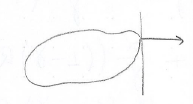
\includegraphics{pic4.png}
\end{figure}

Поскольку $\psi$ "--- внешняя нормаль к $\X$, то $\lambda_5 > 0$, следовательно, положим $\lambda_5 = 1 \thus$
\[
  \left\{
    \begin{aligned}
      &\psi_2(T) = 0,\\
      &\psi_3(T) = 0,\\
      &\psi_1(T) = 1.
    \end{aligned}
  \right.
\]

То есть на последнем участке движения системы будет $u^* = 1$.

Исследуем особый режим: $\psi_1 = \psi_2 \thus$
\begin{gather*}
  0 = \dot{\psi}_1 - \dot{\psi}_2 = -\psi_1u(Ag' - A'g)h - \psi_2 h(1-u)(Ag' - A'g) = \\
  -\psi_1(Ag' - A'g) h[u + 1 - u].
\end{gather*}
$\psi_1 \neq 0$, т.к. иначе $\psi_1 \equiv 0$, а $h() > 0$, значит,
\[
  Ag' = A'g \;\thus\: \dfrac{A(Q)}{A'(Q)} = \dfrac{g(K)}{g'(K)} \;\thus
\]
\[
  \dfrac{1 + Q^{\gamma}}{\gamma Q^{\gamma - 1}} = \dfrac{K^{\alpha}}{\alpha K^{\alpha-1}} \thus K = \dfrac{\alpha}{\gamma}(Q^{1 - \gamma} + Q) \text{ "--- }
\]
вогнутая функция.

$K'_Q = \dfrac{\alpha}{\gamma} + \dfrac{\alpha}{\gamma}(1-\gamma)Q^{-\gamma} > 0$

Продифференцируем $K = \dfrac{\alpha}{\gamma}(Q^{1 - \gamma} + Q)$:
\begin{gather*}
  uAgh - \dfrac{\alpha}{\gamma}\left((1-\gamma)Q^{-\gamma}+1\right)(1-u)Agh \\
  u(1 + \dfrac{\alpha}{\gamma}\left((1-\gamma)Q^{-\gamma} + 1\right)) = \dfrac{\alpha}{\gamma} \left((1-\gamma)Q^{-\gamma} + 1\right) \\
  \thus u_{oc} = \dfrac{\dfrac{\alpha}{\gamma} \left((1-\gamma)Q^{-\gamma} + 1\right)}{1 + \dfrac{\alpha}{\gamma}\left((1-\gamma)Q^{-\gamma} + 1\right)}.
\end{gather*}
Это не статический ОР, при нахождении в нём $K$ и $Q$ изменяются.

Теперь рассмотрим поведение траекторий в конце. Произведём замену независимой переменной: $K = K(t) \to t = t(K)$. Вспомним, что ранее мы показали, что в конце всегда $u = 1$, поэтому
\[
  \dfrac{dQ}{dt} = (1-u) Agh = 0 \;\thus\: Q \equiv \bar{Q},
\]
\[
  \dfrac{dK}{dt} = uAgh = Agh.
\]

\begin{figure}[ht]
  \center
  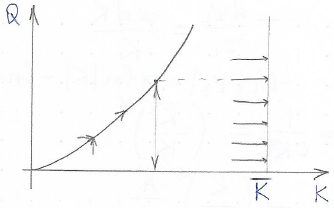
\includegraphics{pic5.png}
\end{figure}

Отсюда
\[
  \dfrac{d\psi_1}{dt} = \dfrac{d\psi_1}{dK} \dfrac{dK}{dt} = \dfrac{d\psi_1}{dK} Agh.
\]
Подставляя $u = 1$ в (СС)
\[
  \left\{
    \begin{aligned}
      &\dot{\psi}_1 = -\psi_1 uAg'h,\\
      &\dot{\psi}_2 = -\psi_1 uA'gh,
    \end{aligned}
  \right.
\]
получим
\[
  \left\{
    \begin{aligned}
      &\dfrac{d\psi_1}{dK} = - \dfrac{\psi_1 g'}{g} = - \dfrac{\psi_1 \alpha}{K}, \\
      &\dfrac{d\psi_2}{dK} = - \dfrac{\psi_1 A'}{A}.
    \end{aligned}
  \right.
\]

Вспомним теперь, что $\psi_1(\bar{K}) = 1$, $\psi_2(\bar{K}) = 0$, получим, проинтегрировав эту систему,
\[
  \psi_1 = \left(\dfrac{\bar{K}}{K}\right)^\alpha,
\]
\[
  \psi_2 = \dfrac{A'(\bar{Q})}{A(\bar{Q})(1 - \alpha)} \left(\bar{K} - K \left(\dfrac{\bar{K}}{K}\right)^\alpha\right).
\]

В какой момент мы переключимся в такой режим движения? В момент, когда $\psi_1 = \psi_2$. Получим описание кривой этого переключения:
\[
  \dfrac{A'(\bar{Q})}{A(\bar{Q})(1 - \alpha)}[\bar{K}^{1 - \alpha}K^{\alpha} - K]\left(\dfrac{\bar{K}}{K}\right)^\alpha= \left(\dfrac{\bar{K}}{K}\right)^\alpha
\]
\[
  \thus \bar{K}^{1 - \alpha} K^{\alpha} - K = \dfrac{(1 - \alpha)A}{A'} = (1 - \alpha) \dfrac{1 + Q^{\gamma}}{\gamma Q^{\gamma - 1}} = \dfrac{1 - \alpha}{\gamma}(Q^{1 - \gamma} + Q),
\]
где $Q = Q(K)$. Продифференцируем последнее соотношение по $dK$, чтобы отыскать точку максимума этой кривой:
\[
  \alpha \bar{K}^{1 - \alpha} K^{\alpha - 1} = 1 \thus K^* = \alpha^{\frac{1}{1 - \alpha}} \bar{K}.
\]
Подставим её в левую часть уравнения кривой:
\[
  \bar{K}^{1 - \alpha} \alpha^{\frac{\alpha}{1 - \alpha}} \bar{K}^{\alpha} - \alpha^{\frac{1}{1 - \alpha}} \bar{K} = \ldots = (1 - \alpha) \alpha^{\frac{\alpha}{1 - \alpha}} \bar{K}.
\]

Тогда
\[
  K^* = \alpha^{\frac{1}{1 - \alpha}} \bar{K} = \dfrac{\alpha}{\gamma}(Q^{1-\gamma} + Q).
\]
Сравнив выражение в правой части с уравнением кривой ОР, построим картину синтеза.

\begin{figure}[ht]
  \center
  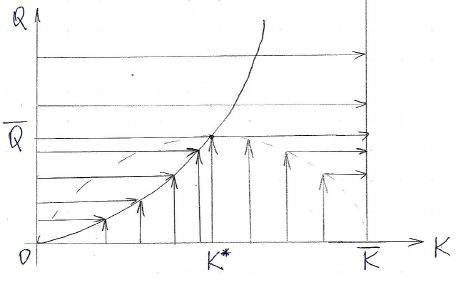
\includegraphics[width=\linewidth]{pic6.png}
\end{figure}

Таким образом, в данном примере движение в особом режиме существенно определяет поведение системы.

\end{document}